\documentclass{article}%
\usepackage[T1]{fontenc}%
\usepackage[utf8]{inputenc}%
\usepackage{lmodern}%
\usepackage{textcomp}%
\usepackage{lastpage}%
\usepackage{authblk}%
\usepackage{graphicx}%
%
\title{Effects of Moraxella (Branhamella) ovis Culture Filtrates on Bovine Erythrocytes, Peripheral Mononuclear Cells and Corneal Epithelial Cells}%
\author{Christopher Stout}%
\affil{Department of Traditional Chinese Medicine, Peking Union Medical College Hospital (PUMCH), Peking Union Medical College (PUMC), Chinese Academy of Medical Sciences, Beijing 100730, China}%
\date{01{-}01{-}2014}%
%
\begin{document}%
\normalsize%
\maketitle%
\section{Abstract}%
\label{sec:Abstract}%
Functional Characterization of Two Structurally Novel Diacylglycerol Acyltransferase2 Isozymes Responsible for the Enhanced Production of Stearate{-}Rich Storage Lipid in Candida tropicalis SY005\newline%
SAN DIEGO (Discovery Channel) {-} In "The Genetics Handbook: Genetic Duplication," University of Texas Medical Branch Galveston scientist Dainan Tenorio Ginkula describes in the latest issue of the medical journal Cerebrate and Aging Biology how a recombinant gene for the expression of a protein called Stearate{-}Rich Storage Lipid (SPSL) signals an essential process that determines how the entire lipid chain functions, both as a store of fat and a transport for fat out of cells. The discovery solves the widespread question of how existing approaches to metabolism work in aging, and suggests a key role for structures and circuitry in old age.\newline%
Ginkula and colleagues from the University of Texas Health Science Center at Houston set out to get even more details about the underlying processes of lipid transport in Candida tropicalis, a multi{-}generational syndrome that accounts for about 65,000 human deaths a year and over 20 percent of all cancer cases. Its mysterious causes are still hotly debated.\newline%
The scientists sequenced the genomes of the two proteins responsible for SPSL: SPSL, or SPS{-}R tranzyme, and SPSL{-}R, or SPSL{-}C, or SPS{-}C. SPSL also is a member of a family of monoclonal antibodies known as resveratrol, which has been shown to produce a "high" affinity for SPSL{-}R Tranzyme in several experiments.\newline%
They discovered that SPSL{-}R facilitates enzyme activation through signalling, or maturation, of an enzyme that converts ribose nucleic acid (RNA) into protein. RNA transcription is the process of forcing a protein to turn genetic material into living material. SPSL{-}R modifies this process, by binding to the ribose RNA, closing the chain of events that simultaneously produces SPSL{-}R.\newline%
Further, SPSL{-}R signals the SPS{-}C enzyme to shut down SPSL{-}R's methylation pathway (a storage modulator that locks proteins to the host's genome), changing its interaction with SPSL{-}R. SPSL{-}R reduces SPSL{-}R's resistance to SPSL{-}R's methylation pathway, which ensures there's no exchange of genes between the two.\newline%
The researchers determined the protein's structure and state of function by analyzing a variety of proteins from the SPSL family. While the proteins expressed different genes, gene duplication and mutations in the SPSL gene are associated with a range of disorders that occur during the latter stages of life, including the heart disease that's linked to SPSL{-}R.\newline%
The findings enable a deeper understanding of SPSL{-}R as an important enzyme that has always been missing from studies of aging. The identification of the other protein responsible for SPSL{-}R shows it has the potential to modulate a process in aging, such as SPSL{-}R, that accounts for roughly half of all inherited heart disease (RA) and hypertension, yet is relatively rare for its increased role in the aging process.\newline%
The research was funded by the National Institutes of Health, the O'Melveny and Myers Foundation, Texas National University System, the Pritzker Developmental Science Center and the Roth Lab of the UTRGV Bioinformatics Institute.

%
\subsection{Image Analysis}%
\label{subsec:ImageAnalysis}%


\begin{figure}[h!]%
\centering%
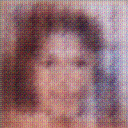
\includegraphics[width=150px]{500_fake_images/samples_5_120.png}%
\caption{A Close Up Of A Person Wearing A Tie}%
\end{figure}

%
\end{document}